\section{High-Level Structure of the \Hybrid}
\label{sec:hybrid.structure}

% \begin{figure}[t]
%     \centering
%     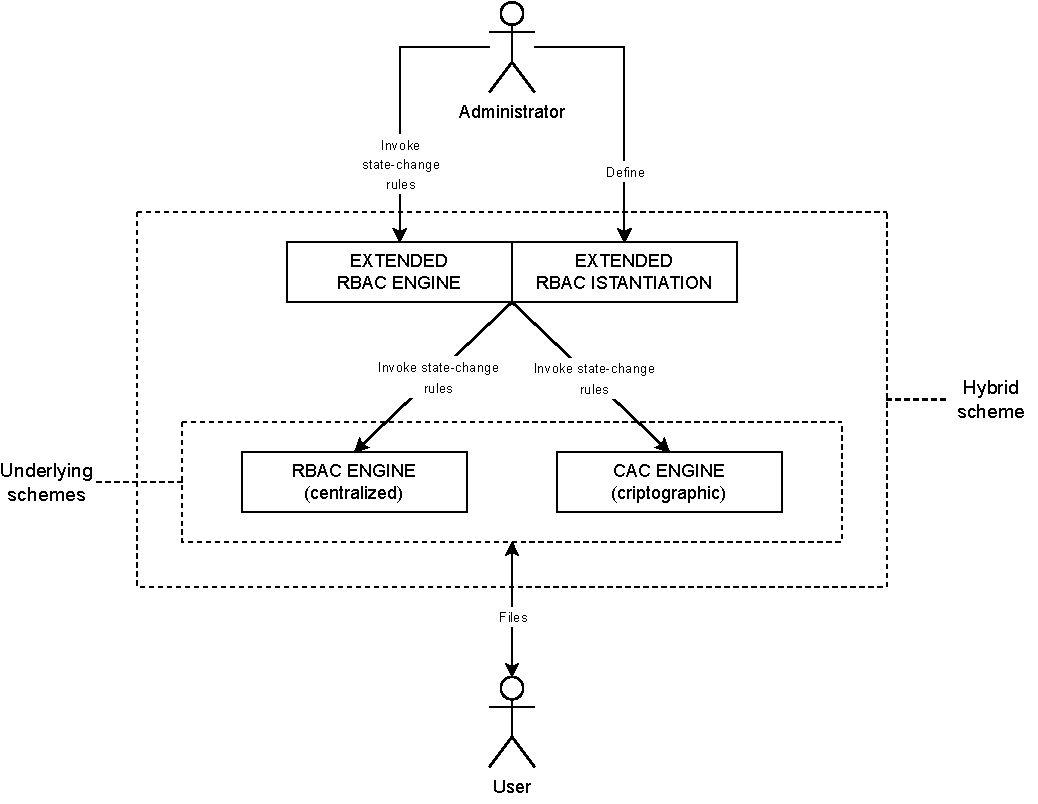
\includegraphics[width=0.75\textwidth]{assets/img/hybrid_scheme.pdf}
%     \caption{\label{fig:hybrid_scheme}The hybrid scheme}
% \end{figure}

Security models typically assume that the \gls{csp} is either completely trusted or honest-but-curious. However, in practice, the actual situation is often somewhere in between, which can allow for more efficient operations and a reduced amount of cryptographic computations. To the best of our knowledge, there is no \gls{ac} \erbacwhat in the literature allowing administrators to specify the security model for their scenario. To this end, we provide an extended \gls{rbac} scheme.
At a high level, the \erbac is automatically compiled into a \centralized and a \cac. The \centralized can be enforced by a traditional \gls{rbac} enforcement mechanisms (e.g., those provided directly by \glspl{csp}). The \cac, as proposed in \cite{cac}, is not able to handle a dynamic security model (e.g., it is not always necessary to re-encrypt a file), so it is necessary to make the changes described in \Cref{sec:background.cac}. The administrator operates on the extended \gls{rbac} model by invoking its state-change rules, which in turn invoke the state-change rules of the centralized \gls{ac} and \gls{cac}, so that enforcement is performed only by these two mechanisms.
To define the security model, we define the concept of predicate, introduce new queries, and modify the entailment as described below.

\paragraph{Predicates.} Predicates are facts, characteristics, or requirements related to users, files, or the \gls{csp}. Predicates are dependent on company processes. For example, if files have different levels of sensitivity, the administrator can introduce a predicate for each level. This results in \( \function{topSecret}(\file) \) for top secret files, \( \function{secret}(\file) \) for secret files, and \( \function{public}(\file) \) for public files. Another example is a company where employees have a smart card that contains the keys \( \keysigu \) and \( \keydecu \) for \gls{cac}, the administrator might want to model the case where the card is lost and all files need to be re-encrypted. To achieve this, a \( \function{lostKeyCard}(\user) \) predicate could be introduced. Our proposal only supports unary predicates, which are predicates applied to a single entity. Although it is possible to introduce predicates on more than one entity, we chose to maintain greater simplicity by only supporting unary predicates.

\paragraph{Queries.} There are several aspects of \gls{cac} that can be customized, and to control each one, new queries were introduced in the \erbac. These queries serve as the interface between the \erbac and the administrator's chosen security model. For instance, the \( \isEncryptionNeededQ \) query determines whether a file should be encrypted or not. \Cref{sec:hybrid.scheme} provides a detailed discussion of queries and their meanings. 


\paragraph{Entailment Instantiation.} The instantiation of the entailment function should result in a \( \mathit{true} \) or \( \mathit{false} \) answer when called with one of the new queries. The answer may be dependent on the predicate assignment. For instance, if a \( \function{confidential} \) predicate exists, the entailment function is instantiated so that when a file \( \file \) has the \( \function{confidential}(\file) \) predicate, the entailment function called with \( \isEncryptionNeededQ \) returns \( \mathit{true} \); \( \mathit{false} \) otherwise.

\Cref{fig:hybrid_structure} illustrates the operations performed in the \hybrid. Specifically, \Cref{fig:hybrid_structure.admin} describes the process an administrator follows when invoking a state-change rule. The proxy receives the invocation and retrieves metadata, including predicates, from the metadata manager. As a result of the execution of the state-change rule --- and according to the retreived metadata --- the proxy updates the centralized \gls{ac} policy and metadata in the metadata manager to reflect the changes in the policy. Finally, it encrypts or decrypts any files for which the protection enforcement mechanism has been altered. \Cref{fig:hybrid_structure.read} illustrates a user reading a file. The user sends a request to the proxy, which retrieves metadata from the metadata manager. The proxy then requests the file from the data manager, which in turn consults the centralized \gls{rbac} mechanism to determine if it can send the file to the user. If authorized, the proxy receives the file and delivers it to the user, decrypting it if necessary. Finally, in \Cref{fig:hybrid_structure.write}, a user writes a file. The plaintext file is sent to the proxy, which retrieves the metadata and determines whether to encrypt the file. If encryption is necessary, the proxy encrypts the file and sends it, along with the new metadata, to the reference monitor. Firstly, the reference monitor retrieves metadata from the metadata manager. Secondly, the reference monitor verifies that the data received from the user is well-formed, checks if the user has permission to write, and ensures that the metadata is consistent. If everything is in order, the metadata is written and the new data is sent to the data manager. The data manager then verifies with the centralized RBAC mechanism whether the user is authorized to write the file. If authorized, the file is written.

% \stefanonote{Non sarebbe male discutere un attimo le figure 3.1a, 3.1b, e 3.1c --- nel senso, spiegare brevemente gli step che vengono effettuati richiamando i concetti introdotti alla fine della Sezione 2.2 (poi non mi sembra diciamo cos'è l'Access Controller; forse meglio rimpiazzare ``Access Controller'' con ``Traditional/Centralized RBAC Enforcement Mechanisms'' o qualcosa di simile?)}


\begin{figure}[t!]
    \centering

    \begin{subfigure}{\textwidth}
        \centering
        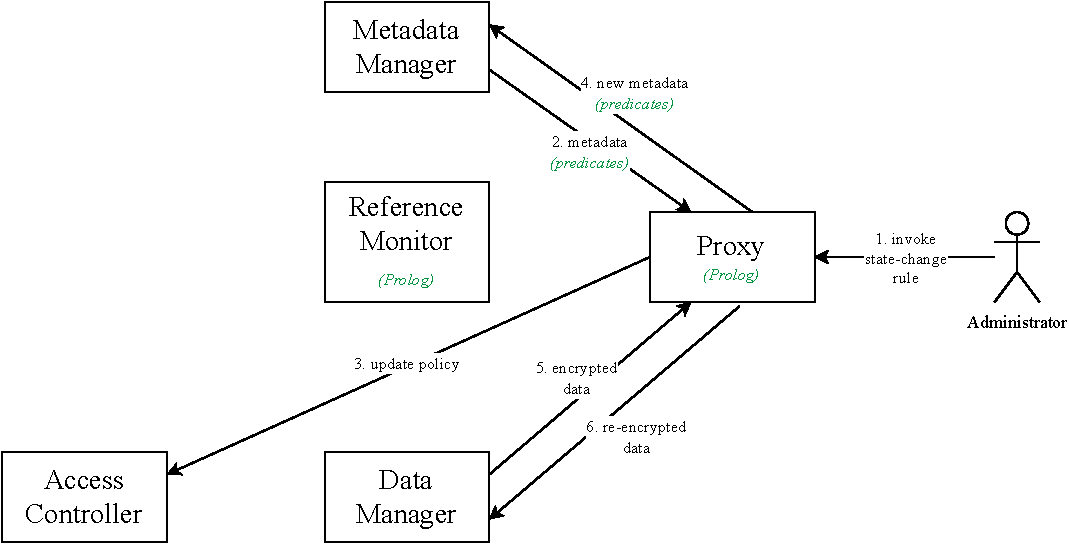
\includegraphics[width=0.7\textwidth]{assets/img2/hybrid_admin.pdf}
        \caption{State-change rule invocation}
        \label{fig:hybrid_structure.admin}
    \end{subfigure}
    \par\bigskip
    \begin{subfigure}{\textwidth}
        \centering
        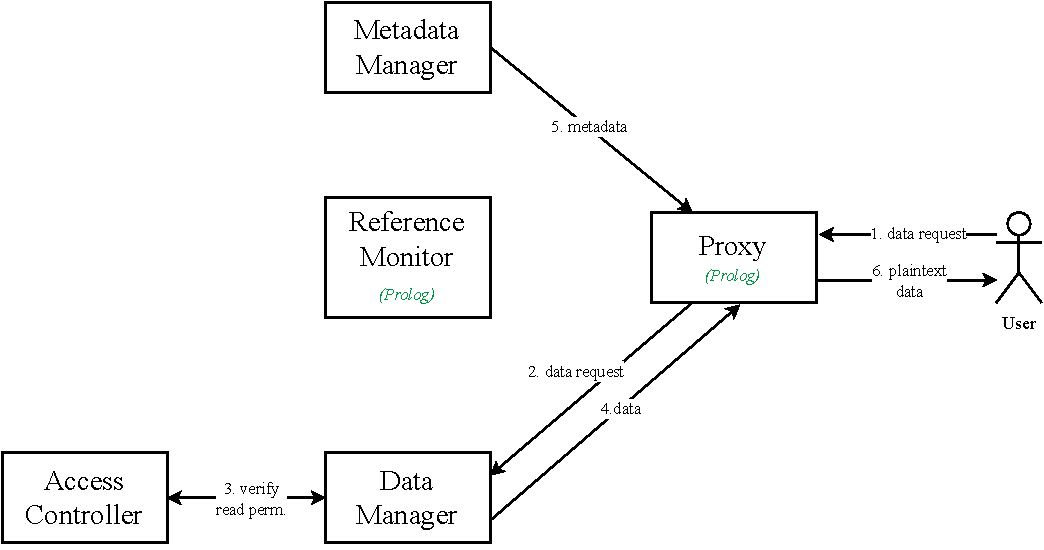
\includegraphics[width=0.7\textwidth]{assets/img2/hybrid_read.pdf}
        \caption{File reading}
        \label{fig:hybrid_structure.read}
    \end{subfigure}
    \par\bigskip
    \begin{subfigure}{\textwidth}
        \centering
        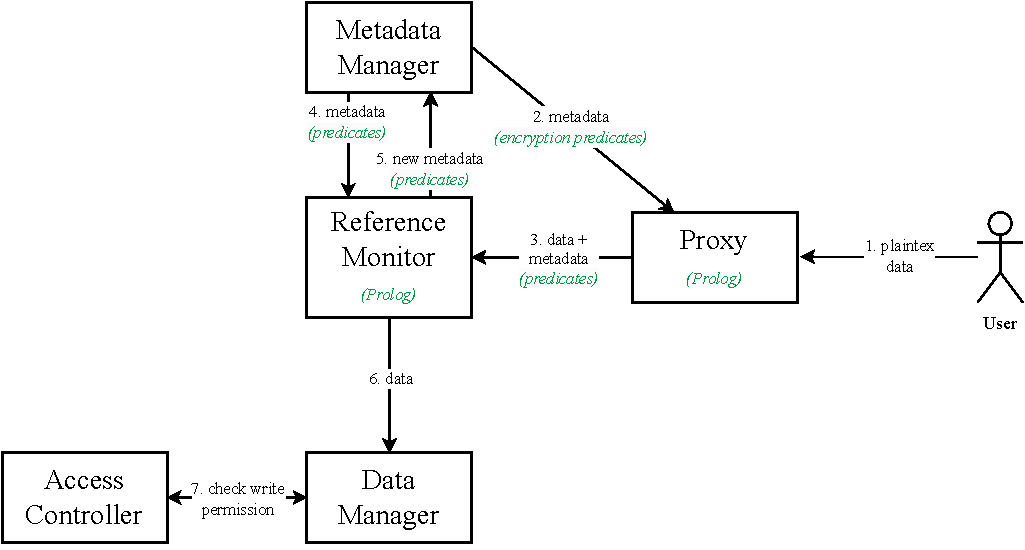
\includegraphics[width=0.7\textwidth]{assets/img2/hybrid_write.pdf}
        \caption{File writing}
        \label{fig:hybrid_structure.write}
    \end{subfigure}

    \caption{Operations In Hybrid Scheme}
    \label{fig:hybrid_structure}
\end{figure}

